\section{Background}
\label{sec:background}

\subsection{AMD XDNA~2 NPU}
\label{subsec:platform}

\textbf{AI Engine Array.}
% VALUE: the array is columns of tiles that run data-driven once configured, so disjoint columns can compute at the same time; a design is one configuration
The AMD XDNA~2 neural processing unit (NPU) in AMD Ryzen\texttrademark{} AI processors contains an array of AI Engine (AIE) tiles in 8 columns~\cite{rico2024xdna,amd_am027}.
Each column holds, from the bottom, a shim tile that moves data between the array and DRAM, a memory tile, and 4 compute tiles, which are VLIW, SIMD vector cores with local memory~\cite{amd_am027}.
Direct memory access (DMA) engines in the tiles move data over a stream switch network, each transfer described by a buffer descriptor (BD), and locks synchronize producers and consumers~\cite{amd_am027}.
A design is one configuration of the array, namely its core programs, stream routes, BDs, and locks, which a compiler such as MLIR-AIE~\cite{hunhoff2025iron,mlir-aie-repo} or MLIR-AIR~\cite{wang2026mlirair} emits.
Once configured, the array executes data-driven: a core runs when its input locks are released, so cores on different columns compute independently whenever their inputs arrive.
% SOURCE: column layout 8 x (shim, memory tile, 4 compute tiles) on the Ryzen AI Max+ 395 NPU, as stated in FCPR Section 2.1 (~/docs/FPGA27__Control_Packet_Reconfiguration.pdf).

\textbf{Command Processor.}
% VALUE: the host reaches the array only through instruction streams that one in-order CP executes; an issue returns at once, a synchronization blocks the CP, so the CP's order decides when each column receives work
The host does not drive the array directly.
Instead, it submits commands, each carrying an instruction stream that the NPU's command processor (CP) executes in order~\cite{rico2024xdna,linux-amdnpu}.
The instructions this work uses are of three kinds.
\emph{Register writes} configure shim BDs and DMA queues, lock values, and runtime parameters in a core's memory.
An \emph{address patch} writes a host buffer's address into a shim BD, where the buffer is named by one of the command's argument slots plus a byte offset.
A \emph{synchronization} blocks the CP until a named DMA transfer signals its completion.
Pushing a BD into a DMA queue returns immediately, so the transfer proceeds while the CP moves on, and we call such instructions \emph{issue} instructions.
Consequently, the CP's instruction order decides when each column receives work, and a synchronization on one column delays every later issue, whichever column it targets.
The NPU can also be divided into partitions of contiguous columns that run independent applications~\cite{rico2024xdna}, whereas the work this paper studies runs in one partition.
Prior work models the time of an array reconfiguration as the CP's critical path, namely its commands and its waits on transfers~\cite{fcpr2027}.
% SOURCE: instruction encoding, mlir-air a3e26261 programming_examples/llms/shared/fused_prefill/insts.py: TXN v1.0 stream; address patch = opcode 0x81 (argument index at word 8, byte offset at word 10); synchronization = opcode 0x80.
% SOURCE: the existing prefill's operators write only shim BDs and queues (row 0, 0x1D000/0x1D200), their own cores' lock registers (0x1F000), and runtime-parameter words in their cores' memory (0x3C00 GEMM, 0x2000 attention); no program loads, core resets, or memory-tile writes (decoded from the shipped streams, lab-prefill-overlap (3)).

\textbf{Host Runtime.}
% VALUE: commands go to a hardware context, run in submission order, bind buffers through a fixed set of argument slots, and each costs a fixed dispatch time that queuing can partly hide
The host submits commands through XRT~\cite{xrt-repo} and the amdxdna driver~\cite{xdna-driver} to a \emph{hardware context}, which holds one configuration of the array.
A hardware context runs its commands in submission order.
Each command binds host buffers to the argument slots that the configuration's kernel declares, and the command's address patches refer to these slots.
Submitting and completing a command costs a fixed time, which we call the \emph{dispatch floor} $F$, independent of the work it carries: an empty command takes about 0.1\ms{} on our platform.
The host can queue further commands before it waits on the first, which hides part of the dispatch floor behind the device's work.
% SOURCE: XRT empty dispatch (4 KB bypass), 93.0-98.5 us at every bracket of lab-prefill-device (3); 92-99 us in lab-prefill-overlap (3).

\subsection{LLM Prefill on the NPU}
\label{subsec:prefill}

\begin{figure}[t]
    \centering
    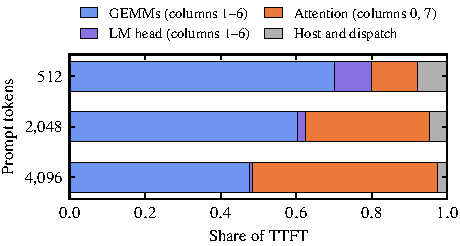
\includegraphics[width=\linewidth]{fig/busy.pdf}
    % VALUE: in the existing prefill, attention's share grows with prompt length, and each column group idles while the other computes
    \caption{Share of time-to-first-token (TTFT) of the existing Llama-3.2-1B prefill by prompt length. Device-busy parts are each operator's time when dispatched alone, less the dispatch floor, summed over the prefill.}
    \label{fig:busy}
\end{figure}

% VALUE: the existing expert prefill already places GEMMs and attention on disjoint columns in one configuration, so its operators differ only in their instruction streams; it runs a layer stage by stage with host work between commands
Prefill processes a prompt to produce the first output token, and its latency is the time-to-first-token (TTFT).
Each decoder layer applies a QKV projection, attention, an output projection, and a gated feed-forward network of gate, up, and down projections.
The open expert prefill of MLIR-AIR~\cite{wang2026mlirair}, laid out like that of FastFlowLM~\cite{fastflowlm-repo}, places every operator of a layer in one configuration, with the GEMMs on columns 1--6 (24 cores) and attention on columns 0 and 7 (one group of 4 cores per column).
Its cores loop indefinitely and take their work from runtime parameters, so its operators differ only in their instruction streams, and each command keeps only the instructions for its own operator's columns.
The prompt is processed in chunks of 128 tokens, and the host runs a layer stage by stage: the QKV projections of all chunks, then each chunk's attention, then each chunk's remaining projections.
The host CPU computes the normalizations, the rotary position embedding, and the residual additions between commands.
% SOURCE: mlir-air a3e26261 programming_examples/llms/shared/fused_prefill/: device.py (column map cols(cfg); "one PDI serves every op and shape and the ops differ only in their insts"), engine.py (strip_columns), dense.py (_mix_all, stage-major order), hostops.py.

% VALUE: the existing prefill issues one operator per command, so its column groups take turns; attention's growing share is time the GEMM columns sit idle
The existing prefill issues one operator per command, which amounts to about 1{,}500 commands for a 2{,}048-token prompt.
Figure~\ref{fig:busy} shows the resulting split of TTFT: device-busy time accounts for 92--97\% of it, and attention's share grows from 12\% to 49\% between 512 and 4{,}096 tokens.
Because the commands run in submission order, columns 1--6 idle while attention runs, and columns 0 and 7 idle while the GEMMs run.
% SOURCE: commands = 16 layers x chunks x 6 + 11 LM-head commands = 1,547 at 2,048 tokens (lab-prefill-census (1)).
% SOURCE: amd-npu e3acc8a prefill-e2/decomp.txt via figs/make_figs.py: busy = isolated time - dispatch floor = 92/95/97% of TTFT at 512/2k/4k; of TTFT, attention 12.2/32.9/49.1%, GEMMs 70.1/60.3/47.6%, LM head 9.7/2.1/0.8%.
% SOURCE: serial execution, the isolated busy times sum to at most TTFT (lab-prefill-device (4)); queued commands do not overlap (Section 3).

% VALUE: packing operators into one dispatch is standard practice for amortizing host overhead; on an in-order CP it does not by itself create concurrency
Placing several operators in one dispatch to amortize per-dispatch overhead is standard practice, as in CUDA Graphs~\cite{nvidia-cudagraphs}, XRT's run lists~\cite{xrt-repo}, and the multi-launch programs that MLIR-AIR stitches together~\cite{wang2026mlirair}.
On the NPU, operators in one command still execute in the CP's instruction order.
Packing therefore removes dispatch cost but creates no overlap unless the operators occupy disjoint columns and the CP issues each one's work before it waits on another's (Section~\ref{subsec:semantics}).
% SOURCE: XRT run list, /opt/xilinx/xrt/include/xrt/experimental/xrt_kernel.h:21 (XRT 2.25.0); MLIR-AIR stitch_elf (vault src-mlir-air-llms).

\subsection{Related Work}
\label{subsec:related}

\textbf{Mapping and Fusion on Spatial Accelerators.}
% VALUE: mapping frameworks choose fused groups and their placement; the designs are separately issued, and their concurrency is not addressed
Stream explores layer-fused mappings on multi-core dataflow accelerators with memory- and communication-aware cost models, and its AIE backend emits one design per fused group~\cite{symons2025stream}.
MLIR-AIR and IRON compile operators and fused multi-operator designs onto the AIE array~\cite{wang2026mlirair,hunhoff2025iron}.
These works decide what a design computes and where, whereas our setting takes the designs as given and concerns how one CP issues them.
% SOURCE: Stream describes no switching cost and no concurrency across fused groups (vault src-stream-dse, arXiv v2 read 2026-10-14).

\textbf{Concurrent Operators on GPUs.}
% VALUE: GPU serving overlaps heterogeneous operators within one device, where the hardware schedules concurrent kernels
NanoFlow splits a batch into nano-batches so that compute-, memory-, and network-bound operations overlap within one GPU~\cite{zhu2025nanoflow}.
On a GPU, kernels on separate streams are scheduled concurrently by the hardware, whereas on the NPU, concurrency must be written into one in-order instruction stream.
% DECISION: the NanoFlow sentence states only what its paper shows; read the PDF and add a vault source note before submission.

\textbf{LLM Inference on AMD NPUs.}
% VALUE: existing NPU LLM runtimes compose hand-tuned designs per model, with the composition fixed by hand
FastFlowLM runs many model families on XDNA~2 NPUs with hand-tuned designs~\cite{fastflowlm-repo}, and MLIR-AIR builds end-to-end decoder models from fused operator designs~\cite{wang2026mlirair}.
In both, the composition of operators into commands is fixed by hand for each model, whereas our setting derives it from the designs' instruction streams.

\textbf{Scheduling with a Shared Server.}
% VALUE: classical scheduling covers machines that share one server and reentrant shops; the CP is a server that also blocks on completions
Scheduling theory studies parallel machines whose jobs each need a common server for setup~\cite{hall2000common,glass2000dedicated}, and reentrant shops in which jobs return to a machine several times~\cite{wang1997reentrant}.
The CP resembles such a server, with the difference that it also blocks on synchronizations until a machine's work completes.
% DECISION: these three works are cited from their metadata only; read each PDF and add a vault source note before submission.
